\documentclass[a4paper,12pt]{article}
\usepackage{amsmath,amsfonts,amssymb}
% \usepackage{geometry}
\usepackage{fancyhdr}
\usepackage{graphicx}
\usepackage{titlesec}
\usepackage{xcolor}
\usepackage{tikz}
\usepackage{tcolorbox}
\usepackage{float} % For figure positioning
\usepackage{lipsum}
\usepackage[utf8]{inputenc}
\usepackage[a4paper,hmargin=0.8in,bottom=1.5in]{geometry}
\usepackage{hyperref}
\usepackage{fancyhdr}
\usepackage{textgreek}
\usepackage{graphicx}
\usepackage{subcaption}
\usepackage{mathrsfs}
\usepackage{enumitem}
\usepackage{amsmath}
\usepackage{amsthm}
\usepackage{mathtools}
\usepackage{multirow}
\usepackage{listings}
\usepackage{cancel}
\usepackage{amssymb}
\usepackage{listings}
\usepackage[english]{babel}
\hypersetup{colorlinks=true, linkcolor=black, urlcolor=magenta}
\geometry{margin=0.5in}
\pagestyle{fancy}
\lstset{ 
    language=Python,
    basicstyle=\ttfamily\small,
    keywordstyle=\color{blue},
    stringstyle=\color{red},
    commentstyle=\color{green},
    morekeywords={self}, 
    frame=single,
    breaklines=true,
    showstringspaces=false
}
\fancyhf{}

% Header and Footer
% \fancyhead[L]{\includegraphics[width=1.5cm]{logo.png}} % Add your logo
% \fancyhead[C]{\textbf{\color{blue!70}CS378-LAB3}}
% \fancyhead[R]{\color{blue!70}Saksham Rathi \\ \today}
\fancyfoot[C]{\thepage}

% Custom Section Color and Format
\titleformat{\section}
{\color{purple!80!black}\normalfont\Large\bfseries}
{\thesection}{1em}{}


% Beautiful Title with TikZ
\newcommand{\cooltitle}[1]{%
  \begin{tikzpicture}
    \node[fill=blue!20,rounded corners=10pt,inner sep=10pt] (box)
    {\Huge \bfseries \color{black} #1};
  \end{tikzpicture}
}

% Stylish Solution Environment with float option enabled
\newtcolorbox{solution}[2][]{colframe=green!60!black, colback=green!5!white, 
    title=#2, fonttitle=\bfseries\large, float=htbp}

\title{\cooltitle{CS378 Lab-3 Design Doc}}
\author{{\bf Saksham (22B1003), Dion (22B0029), Geet (22B1035), Kavya (22b1053)} \\
\small Department of Computer Science \\
Indian Institute of Technology Bombay}
\date{September, 2024}

\begin{document}
\maketitle
\section{Physical Layer}
\subsection{Preamble}
In order to maintain the reliability and accuracy of signal transmission, we use a preamble. A preamble is a pre-defined sequence of bits transmitted at the beginning of the signal. 

In our assignment, the preamble is generated as a sine wave at a distinct frequency, different from those used for transmitting the actual data. This frequency difference allows the receiver to easily identify the preamble and differentiate it from the main message. The preamble is transmitted 6 times, with each one having a short bit duration of typically around 0.02s. This extended transmission time helps the receiver lock onto the signal and synchronize accurately, ensuring that the actual data that follows is received without errors.

\subsection{Synchronization}
During signal transmission, synchronization between the sender and the receiver is of utmost importance to make sure that the message is correctly interpreted. Proper synchronization ensures that the receiver correctly aligns its listening window with the sender's bit transmission. Without synchronization, even small timing discrepancies can lead to significant errors in interpreting the transmitted data. To put this into perspective, consider the case where the sender is transmitting the sequence 
\texttt{101001}, where each bit duration is 0.3 seconds. If the receiver starts listening at the wrong time—let's say, 0.4 seconds late—it can miss the first bit, and may not correctly identify the upcoming bits. In real situations, errors due to improper synchronization are quite common. So we address this as follows:

For this, we employ a preamble and design the receiver to detect changes in the transmitted bits. The preamble has a bit duration of approximately 0.02 seconds, while the actual message bits transmitted by the sender have a much longer duration of around 0.3 seconds. The short duration of the preamble relative to the bit duration allows for a degree of tolerance—any slight delay or variation in detecting the preamble will not significantly impact the timing of the subsequent bit transmission.

Once the receiver detects and identifies the preamble, it becomes synchronized with the sender and is prepared to receive the actual data. The longer bit duration ensures that even if there are minor discrepancies in timing, the receiver can still correctly interpret the data. 

\subsection{Error Correction}
We use a \textbf{CRC based} algorithm to check for errors using redundant bits. Our CRC generator polynomial is \textbf{0x5d7}, chosen from \href{https://users.ece.cmu.edu/~koopman/crc/index.html}{this online compendium on CRCs} (We chose the minimum HD to be $5$ to be able to detect upto $2$ errors.)
\subsubsection{Encoding algorithm}
As is standard in CRC codes, we use a \verb|crc_remainder|  function that finds the remainder of the input bitstring (appended with (length of generator polynomial - 1) zeroes to the right of it) with the generator polynomial
\newline This \verb|crc_remainder| function does normal long division over the Galois Field $GF(2)$
\newline The pseudocode for the \verb|crc_remainder| function is as follows - 
\begin{verbatim}
crc_remainder(bit-string input, bit-string generator_polynomial):
    let L <- length(generator_polynomial)
    let augmented_code <- input appended with (L - 1) zeros to the right
    for bit i in augmented_code:
        if bit i is 1 and there are atleast (L-1) bits to the right of i:
            XOR the next L bits (including bit i) of augmented_code with generator_polynomial
    return augmented_code 
\end{verbatim}
Our final encoding algorithm is as follows - 
\begin{verbatim}
encode_crc(bit-string input, bit-string generator_polynomial):
    let rem <- crc_remainder(input, generator_polynomial)
    return (input appended to rem)
\end{verbatim}
The fact that our polynomial has degree $11$ and our message length can go upto $20$ means that our transmitted message can go upto $31$ bits in length
\newline Along with the $6$ bits in the preamble, the total message length goes up to $37$ bits
\subsubsection{Decoding and Error Correcting Algorithm}
Our decoding algorithm is a trial-and-error algorithm that works as follows (and uses the fact that there can be atmost $2$ errors in the transmitted message):
\begin{verbatim}
decode(bit-string transmitted_message, bit-string generator_polynomial):
    // Assume no error for now
    if(crc_remainder(transmitted_message, generator_polynomial) == 0):
        return transmitted_message // No error
    // Assuming 1 error now
    for(bit i in transmitted_message):
        augmented_message <- transmitted_message with bit i flipped
        if(crc_remainder(augmented_message, generator_polynomial) == 0): 
            return transmitted_message // 1 error
    // Now it has to be 2 errors
    for(bit i and j in transmitted_message):
        augmented_message <- transmitted_message with bits i and j flipped
        if(crc_remainder(augmented_message, generator_polynomial) == 0): 
            return transmitted_message // 2 errors
\end{verbatim}
\subsubsection{Testing}
In addition, we tested our code for every possible error and made sure that it actually works as well. Our testing code is as follows - 
\begin{verbatim}
tester():
    for l from 1 to 20:
        generate all bitstrings of length l
        for bitstring in sequence of bitstrings:
            msg <- bitstring
            intended_msg <- encode_crc(msg, generator_polynomial)
            for i, j in length(intended_msg):
                augmented_msg <- intended_msg with i and j bits flipped
                assert(decode(augmented_msg) == intended_msg)
\end{verbatim}
In addition, we tested that there is one and only one valid message corresponding to a corrupted message

\subsection{Some Finer Details}
The bits - 0 and 1 are being transmitted at different frequencies which are 4000Hz and 6000Hz respectively. The preamble is being transmitted at 8000Hz. The sender sends a particular bit for 0.3 seconds. The receiver detects frequencies in every interval of 0.05 seconds. So, basically the receiver expects that the window length of a particular frequency will be 6, for it to decide on the bit which was transmitted. Through such a mechanism, we ensure that the synchronization delay is compensated, and we receive the correct bitstring. We stop the receiving side, when we receive three `?' (which do not correspond to the frequencies of 0 and 1).


\section{MAC Layer}

\subsection{Introduction}
We plan to implement CSMA-CA (which is also used in WiFi) with some modifications to handle some specific cases. \textcolor{red}{\bf 
 We plan to carry out our demo using 3 laptops.}

\subsection{Frame Structure}
Here are the allotted addresses to the nodes:
\begin{itemize}
    \item {\bf ``00"}: All nodes (1, 2, 3). This bitset will be used for broadcast purposes. Clearly, this bitset can't be in the sender's address field, but it can be present in the receiver's address field.
    \item {\bf ``01"}: Node-1
    \item {\bf ``10"}: Node-2
    \item {\bf ``11"}: Node-3
\end{itemize}

The sender will initially send an RTS (request-to-send) frame. The structure of this will be as follows:
\begin{center}
    \begin{tabular}{|c|c|c|c|}
    \hline
    \textbf{Field} & \textbf{Size (bits)} & \textbf{Description} \\ 
    \hline
    Preamble & 6 & To synchronize everybody  \\ 
    \hline
    Sender's Address & 2 & Address of the sender \\ 
    \hline
    Receiver Address & 2 & Address of the receiver\\ 
    \hline
    % Length of the message & 4 & Length of the message which will be sent in the data frame \\ 
    % \hline
    \end{tabular}
\end{center}

If the RTS is received (and decoded successfully by the receiver), then it will send a CTS (clear-to-send) which has similar structure as follows:
\begin{center}
    \begin{tabular}{|c|c|c|c|}
    \hline
    \textbf{Field} & \textbf{Size (bits)} & \textbf{Description} \\ 
    \hline
    Preamble & 6 & To synchronize everybody  \\ 
    \hline
    Sender's Address & 2 & Address of the sender \\ 
    \hline
    Receiver Address & 2 & Address of the receiver\\ 
    \hline
    % Length of the message & 4 & Length of the message which will be sent in the data frame \\ 
    % \hline
    \end{tabular}
\end{center}


If the CTS is received successfully by the original intended sender, it will send the data frame which has the following structure:
\begin{center}
    \begin{tabular}{|c|c|c|c|}
    \hline
    \textbf{Field} & \textbf{Size (bits)} & \textbf{Description} \\ 
    \hline
    Preamble & 6 & To synchronize everybody  \\ 
    \hline
    Sender's Address & 2 & Address of the sender \\ 
    \hline
    Message ID & 2 & A unique identifier to each message being sent\\ 
    \hline
    Length of the message & 4 & Length of the message which will be sent in the data frame \\ 
    \hline
    Data & 1-15 & The message itself \\ 
    \hline
    % Ending-Preamble & 4 & To signify that the channel is now free\\ && and can be used for further transmission \\ 
    % \hline
    \end{tabular}
\end{center}

Above \textbf{Message ID} is a unique 2-bit identifier assigned a unique 2-bit identifier. Since only 4 bits in total need to be transmitted, a 2-bit identifier is sufficient. This ensures that the receiver does not redundantly decode the same message multiple times. \\

Once the receiver successfully receives the message, it sends a 2-bit \textbf{Acknowledgement} using a specific frequency to confirm proper reception and indicate the absence of any collision.
% Since, the devices are kept nearby, we do not plan to send ACK (acknowledge) frame. This will help us increase the overall efficiency.

\subsection{Flow-chart}
\begin{figure}
    \centering    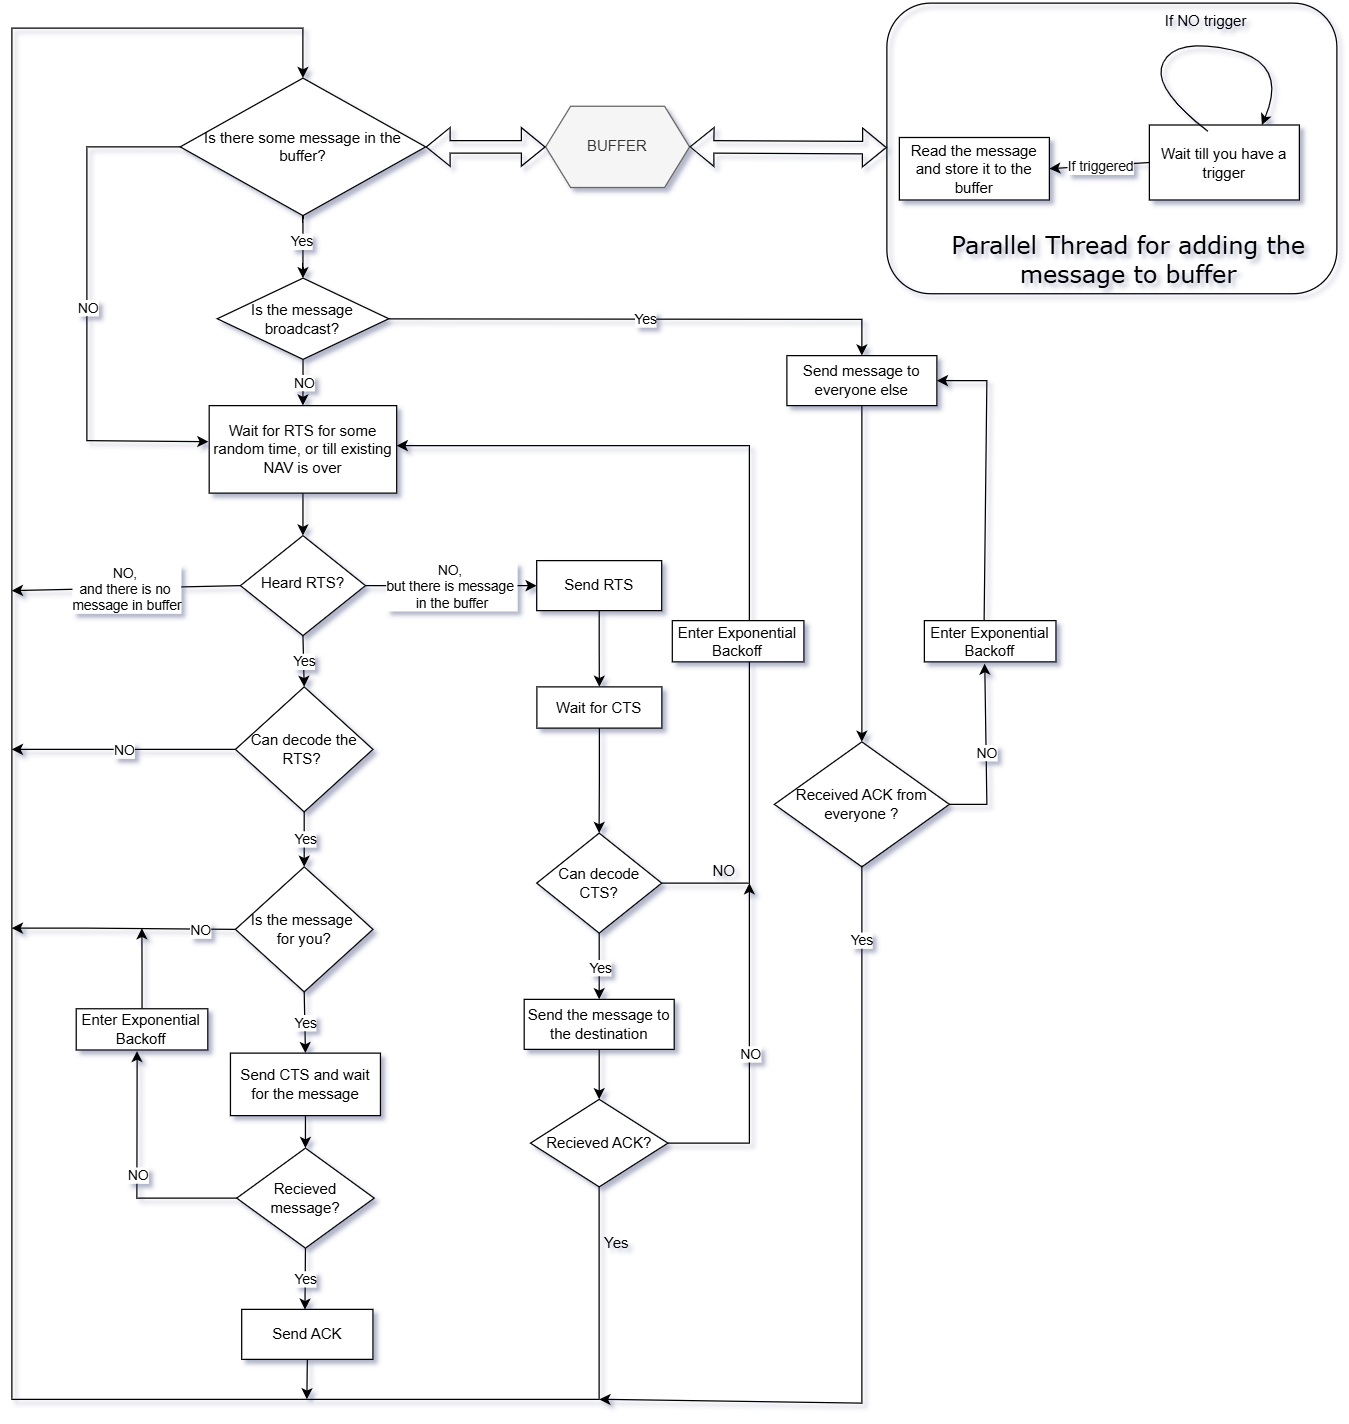
\includegraphics[width=\textwidth]{fig.png}
    \caption{Flow Chart for MAC Layer Implementation}
    \label{1}
\end{figure}

Figure \ref{1} presents the flow chart of our overall implementation. Our MAC Layer is primarily built on the standard \textbf{CSMA-CA} mechanism (similar to WiFi) but with some specific modifications tailored for our protocol.

Our design uses two threads running in parallel. One thread is responsible for adding incoming messages to a buffer whenever a trigger is activated. The second thread, which is the \textit{main protocol implementation}, handles the communication process based on these buffered messages.

In the \textit{main thread}, each node first checks whether its buffer contains a message to be transmitted. If a message exists, the node identifies if it is a \textbf{broadcast} message. Broadcast messages follow a distinct procedure: the node sends the message directly and waits for acknowledgments from all nodes. If any acknowledgment is missing, it re-sends the broadcast message after applying an \textit{exponential backoff}. When all acknowledgments are successfully received, the node reverts to checking its buffer for any new messages.

For \textbf{non-broadcast} messages, the node checks if an \textbf{RTS} (Request to Send) has been transmitted or if the ongoing \textbf{NAV} (Network Allocation Vector) period is active. If the NAV is still active, the node waits until it expires before running the exponential backoff algorithm and sending its RTS. If no NAV is set, the node waits for a random backoff interval and then transmits its RTS.

While listening for \textbf{incoming RTS messages}, if the node detects an RTS not meant for itself, it simply returns to checking the buffer and waits. However, if the RTS is directed to the node, it responds with a \textbf{CTS} (Clear to Send) and then waits for the data frame. Upon receiving the data frame successfully, it sends an acknowledgment and reverts to checking the buffer. If no data frame is received after sending the CTS, the node assumes a \textbf{collision} and triggers an exponential backoff.

Meanwhile, the sender, after transmitting its RTS, waits for a corresponding CTS. If no CTS is received, the sender assumes a collision and performs an exponential backoff before reattempting to transmit the RTS. Upon successfully receiving the CTS, the sender sends the \textbf{data frame} and waits for an acknowledgment. If the acknowledgment is successfully received, it returns to the buffer-checking stage; otherwise, it considers a collision occurred and engages in exponential backoff.

If the buffer is empty, the node simply waits for incoming RTS messages. Upon detecting an RTS, it engages in the standard \textsf{CTS-Message-ACK} sequence described above. If no RTS is detected, it returns to monitoring its buffer and waiting for new events.


\subsection{Some Implementation Details}
Here are some of the points relating to implementation details:
\begin{itemize}
    \item We will synchronize the clocks using NTP protocol.
    \item We plan to send each frame in multiples of 4 (4 bits together). Total 16 such sets will map to 16 different frequencies.
    \item RTS, CTS, Preamble have different frequencies to make it easy to detect for the nodes.
    \item The exponential backoff will be iniated with a range $\Delta \in {1, 2}$. And after each unsuccessful trial, the range will double the previous size. Each element of the range will have equal probability of occurring.
    \item The time $\Delta$ will be set equal to one bitset-duration (bitset contains 4 bits in each case).
    \item We need to maintain various variables at each node such as the number of unsuccessful trials, whether a transmission is going on etc.
    \item We plan to maintain the buffer as some file (which will map to stdin of the current code). So, a single code file will be involved both in taking inputs and also in the transmission process.
\end{itemize}

\subsection{Algorithm}
\begin{enumerate}
    \item We input the node-id 
    \item Then, we check if we have any messages to send. If so, then we read it into a buffer and if not then we just wait and listen for the RTS or until the existing NAV is over.
    \item Note - If we have a message then we read it and store it into the buffer (This is a parallel running thread)
    \item If we have a message we check if it's a broadcast and send it to the other nodes as per the receiver(s)
    \item For sending, we first wait for RTS for some random time or till existing NAV is over
    \item If we have heard the RTS and cannot decode it we start the whole process again
    \item Else if we have heard the RTS and can decode it and the message is for us, then we send the CTS and wait for the message
    \item If we receive the message we send the Acknowledgement and if not then we enter exponential backoff (Max wait time = Max wait time $\times$ 2)
    \item Also, if we haven't heard the RTS and have a message in the buffer, we send the RTS and wait for CTS.
    \item If we cannot hear or decode CTS, we again enter exponential backoff 
    \item If we can decode the CTS and it is meant for us, then we send the message to the destination and wait for the Acknowledgement. If we don't receive the Acknowledgement, we again go into exponential backoff and repeat the process
\end{enumerate}

\subsection{Pseudo code}
\begin{lstlisting}
    Node id <- input node id
    while True:
        if we have message to send:
            load message into buffer
        Check frequency running in the environment
        if frequency is broadcast (someone wants everyone to hear it):
            Check for preamble
            if we havent heard preamble (timed out):
                continue
            Receive the message
            if we are not able to decode correctly:
                continue
            Add message to output
            Send acknowledgement
        else if frequency is preamble:
            Try to listen for preamble
            if time out (cannot listen to preamble):
                continue
            Check if message is meant for us
            if message is meant for us:
                Receive the message
                if we are not able to decode correctly:
                    continue
                Add message to output
                Send acknowledgement
            else:
                Wait for acknowledgement until NAV is over
        else:
            if sender has message to send and waiting period is over:
                if message is broadcast:
                    Send preamble
                    Send message
                    Wait for CTS 
                    if CTS is heard:
                        Send message
                        Wait for acknowledgements
                        if Acknowledgements are heard:
                            Update buffer
                            continue
                        else:
                            continue after updating number of collisions
                    else:
                        continue after updating number of collisions
                Send the preamble
                Send the message
                Wait for CTS 
                if CTS is heard and it is for us:
                    Send message
                    Wait for acknowledgement
                    if Acknowledgement is heard:
                        Update buffer
                        continue
                    else:
                        continue after updating number of collisions
                else:
                    continue after updating number of collisions
\end{lstlisting}

 Note that the maximum waiting period is dependent on the number of collisions ($2^{\text{num\_collisions}}$)
\subsection{Testing}
We have built our protocol to be able to scale to any number of nodes. For the testing, we will be doing it with \textbf{3 nodes (laptops)}

\subsection{Instructions for Running}
The following have to be done one after the other (in parallel terminals):
\begin{enumerate}
    \item python3 input.py (this file is for inputting the messages, an enter from the user acts as a trigger and the MAC layer will try to send that message as soon as possible)
    \item python3 main.py (this file is for receiving and sending the messages; initially it expects the node id as input (1, 2, 3))
\end{enumerate}
\end{document}